\chapter{Integration Tests}

\section{Test case scenarios}
\begin{table}[H]
    \begin{tabular}{|l|l|l|p{10cm}|}
    \hline
    Case & Control Unit & Unit under Test & Execution \\ \hline
    1 & CDU & Sensor & CDU sends a get info request to a sensor. \\ \hline
    2 & Sensor & CDU & Sensor sends info to the CDU \\ \hline
    3 & PC & CDU & PC sends a get data request to the CDU \\ \hline
    4 & CDU & Sensor & CDU requests data from a sensor that does not exists \\ \hline
    5 & PC & CDU & PC sends a message to the CDU that the CDU does not recognise. \\ \hline
    6 & Sensor & CDU & Sensor sends invalid data to the CDU \\ \hline
    7 & Sensor & CDU & CDU sends a get data request to a sensor but does not allow the sensor to respond. \\ \hline
    8 & Sensor & CDU & CDU sends a get data request to a sensor. The sensor responds but occupies the bus and never lets go. \\ \hline
    \end{tabular}
\end{table}

\section{Test case results}
\begin{table}[H]
    \begin{tabular}{|l|l|l|p{10cm}|}
    \hline
    Case & Expected result & Actual result & Done \\ \hline
    1 & ~ & ~ & ~\\ \hline
    2 & ~ & ~ & ~\\ \hline
    3 & ~ & ~ & ~\\ \hline
    4 & ~ & ~ & ~\\ \hline
    5 & ~ & ~ & ~\\ \hline
    6 & ~ & ~ & ~\\ \hline
    7 & ~ & ~ & ~\\ \hline
    8 & ~ & ~ & ~\\ \hline
    \end{tabular}
\end{table}

\begin{figure}[H]
\centering
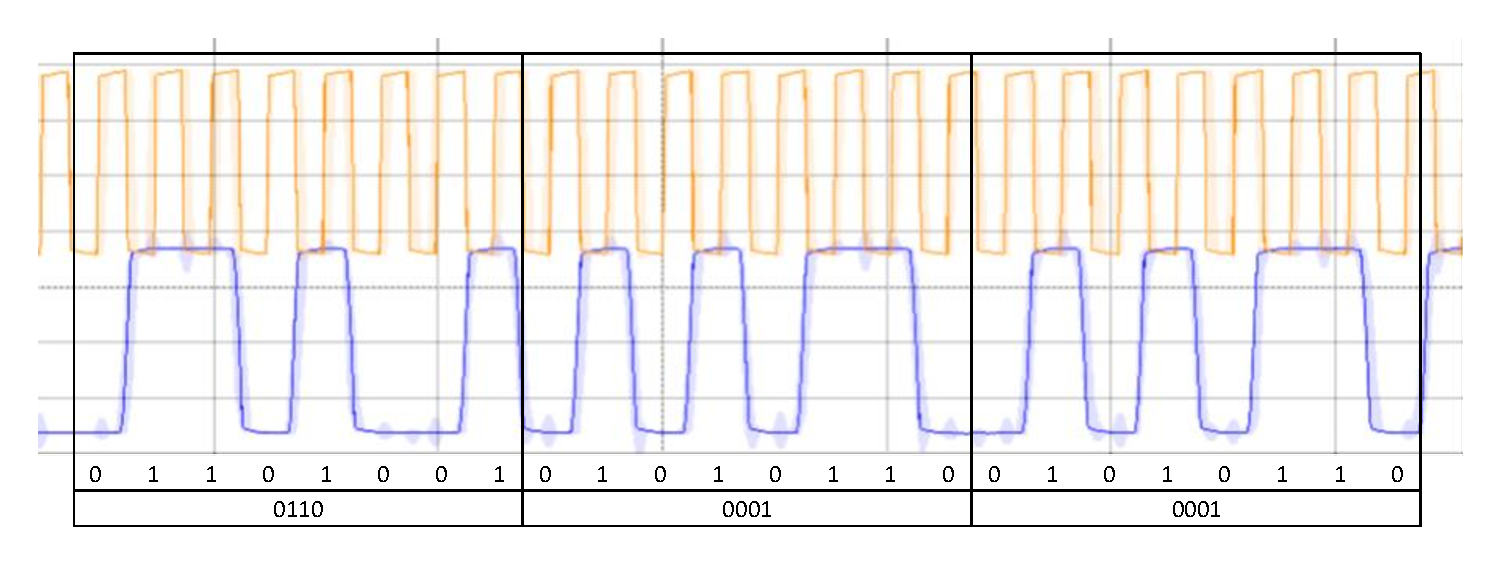
\includegraphics[width=0.5\textwidth]{billeder/CDUtestcase9}
\caption{Test Case 1 Result}
\label{fig:InteTestCase1}
\end{figure}

